\documentclass[10pt]{article} % Default font size is 12pt, it can be changed here
\usepackage{geometry} % Required to change the page size to A4
\geometry{a4paper}\usepackage[utf8]{inputenc}
\usepackage[dutch]{babel}
\usepackage[T1]{fontenc}
\usepackage{titling}
\usepackage[hyphens]{url}
\usepackage{hyperref}
\usepackage{graphicx}

\hyphenation{school-vakanties}

\setlength{\droptitle}{-11em}   % This is your set screw

\title{COVID-19 vier keer sneller en eenvoudiger ontcijferen}
\author{}
\date{}

\begin{document}

\maketitle

\vspace{-70px}
\noindent \textbf{Vanaf dat COVID-19 de wereld heeft overgenomen, komen zowel onze regering als de wereldgezondheidsorganisatie (WGO) constant raad vragen bij de wetenschappers van ons land voor meer informatie over wat ze moeten doen. Deze informatie verkrijgen ze door COVID-19 los te laten op de Belgische bevolking in een computersimulatie, om zo te kunnen voorspellen wat er gebeurt als we bijvoorbeeld 1,5 meter afstand houden of de scholen sluiten. Om veel sneller en makkelijker voorspellingen te kunnen doen, heb ik zo een computerprogramma (genaamd Stride) onder handen genomen waardoor een simulatie van twee uur nu minder dan een halfuur duurt, en waardoor zelfs u ons kan simuleren.}
\\\\
Vooraleer de overheid besliste om onder andere mondkapjes verplicht te maken en om de schoolvakanties te verlengen, is er veel onderzoek gedaan naar het effect van deze maatregelen. Hiervoor deden ze beroep op de onderzoekers van ons land die kunnen inschatten wat de gevolgen zijn van zulke maatregels en of ze wel degelijk nuttig zijn. Dit doen ze door computerprogramma's te gebruiken die simuleren hoeveel mensen besmet worden van de 11 miljoen Belgen. Zo een simulaties kunnen al snel enkele uren duren, desondanks dat ze uitgevoerd worden op de krachtigste computers van ons land in het Vlaams Supercomputer Centrum (VSC). Het virus wachtte op niemand, dus hebben de regering en onderzoekers telkens zo snel mogelijk beslissingen moeten maken. Door mijn aanpassingen verlopen de simulaties uiteindelijk 4,5 keer sneller. Hoe meer en sneller simulaties ze dus kunnen uitvoeren, hoe beter en hoe meer maatregelen ze kunnen beoordelen.

\subsection*{Een dag in de simulatie}
Elke belg zit in meerdere bubbels, zoals zijn huishouden, werk of school, vrije tijd, etc. Voor elke dag in een simulatie moet er berekend worden wie met elkaar contact heeft en wie elkaar besmet in elke bubbel. Dit zorgt er echter wel voor dat we dagelijks 11 miljoen mensen moeten volgen die onderling allemaal contact hebben in verschillende bubbels, wat al snel kan oplopen tot miljarden berekeningen per dag. Met de informatie dat we hiermee genereren, kunnen we bijvoorbeeld te weten komen hoeveel contacten iedereen per dag gemiddeld heeft afhankelijk van de maatregelen. Dit helpt ons om in te zien waar we de meeste kans hebben op besmetting, of we kunnen voorspellen hoeveel werk contact tracers zullen hebben.
\\\\
{\Large``Één teken toevoegen in meer dan 44 000 regels code verdubbelt bijna de snelheid.''}
\\\\
Het hele programma bevat meer dan 44 000 regels code, wat ontzettend veel is om te analyseren en om er verbeteringen in te vinden. Ik heb ontdekt dat de manier waarop het programma geschreven was, achterliggend telkens een heel klein beetje extra werk deed. Dit extra werk kost amper tijd als het één keer uitgevoerd moet worden (ongeveer 1 nanoseconde wat 0,000000001 seconden is). Het probleem was echter dat dit stukje extra werk werd uitgevoerd voor de berekening van elk contact. Zoals ik daarnet al zei, zijn er miljarden contacten die berekend moeten worden per dag. Een simulatie duurt meestal meer dan 100 dagen, dus al die kleine beetjes tellen uiteindelijk op tot een groot geheel. Door één teken toe te voegen (een ampersand `\&') in al die regels code, voorkom ik dat dit extra beetje werk uitgevoerd wordt. Dit leidde uiteindelijk al tot bijna een halvering van de tijd door enkel de code goed te bestuderen, wat ondertussen al meer dan een halfjaar wordt toegepast in de praktijk.

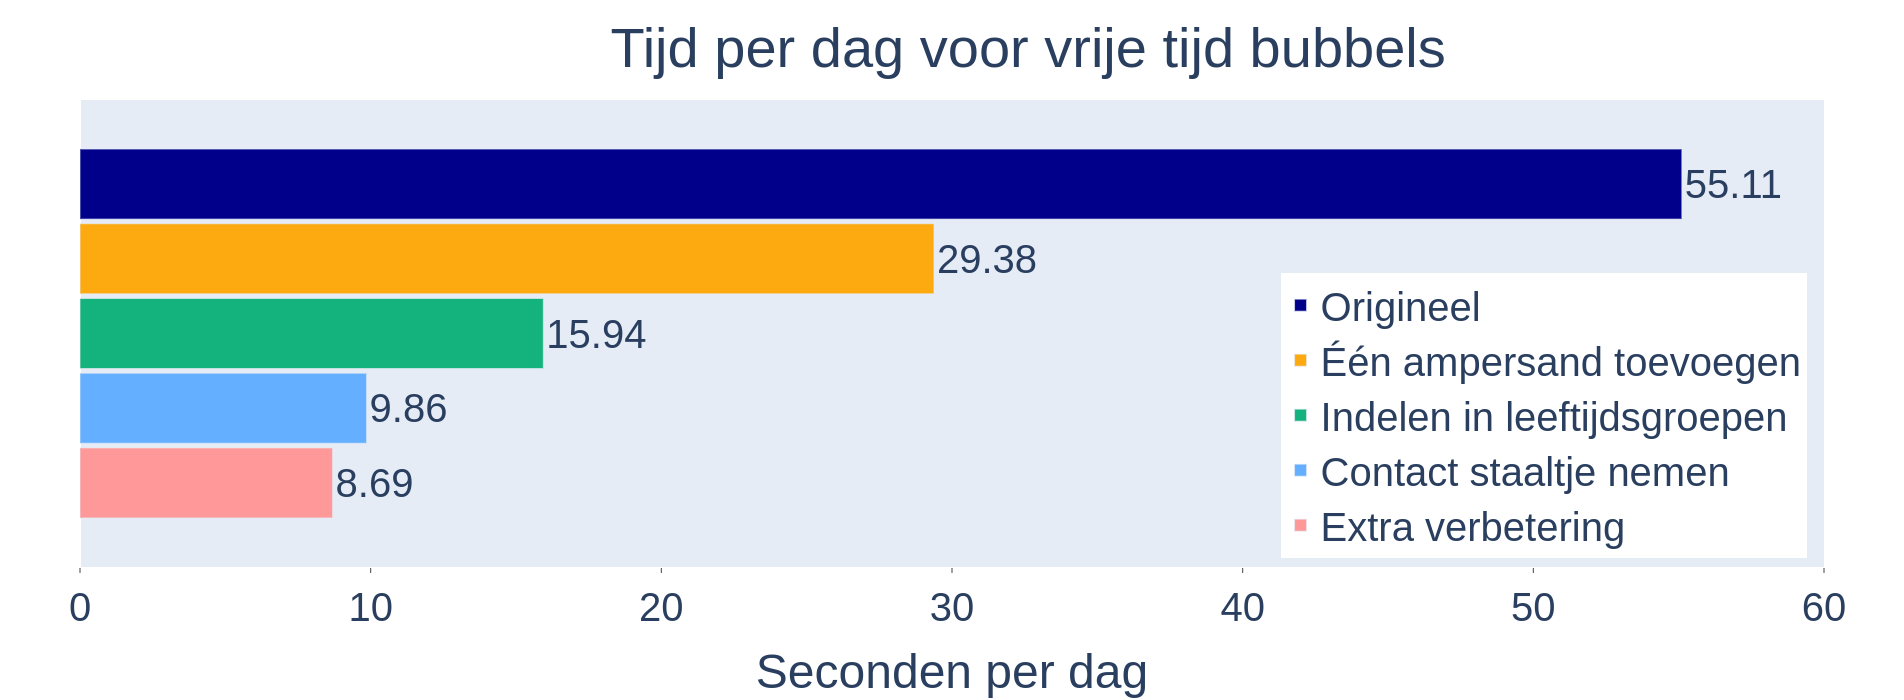
\includegraphics[width=\linewidth]{snelheidswinst.png}

\subsection*{5 miljoen huishoudens stellen niks voor}
Om te berekenen wie allemaal met elkaar contact hebben, gaat het programma iedereen in een bubbel met elkaar matchen. Als u bijvoorbeeld met 2 collega's Daan en Amber werkt, worden er 3 matches bekeken: jij met Daan, jij met Amber, en Daan met Amber. Wanneer u samenwerkt met 10 collega's, moeten er dus (10+9+8+...+1=) 55 paren van personen bekeken worden om te kijken als ze contact hebben. Als we nu willen uitdrukken hoeveel paren er berekend moeten worden voor een bubbel, kunnen we dit doen door het kwadraat te nemen van het aantal personen in de bubbel. Dit is niet 100\% correct (want $10^{2} = 100$ en $3^{2} = 9$), maar het geeft wel de impact weer van de grootte van een bubbel. We zeggen dan ook dat het programma kwadratisch meer tijd kost voor grote bubbels dan voor kleinere.
\\\\
{\Large ``Een bubbel van 50 man is 100 keer duurder dan eentje van 5.''}
\\\\
Huishoudens bevatten gemiddeld 2-3 personen, waardoor heel snel contacten berekend kunnen worden tussen gezinsleden. Vrije tijd bubbels kunnen echter tot bijna 1 500 mensen bevatten, wat er dus voor zorgt dat ze gigantisch meer in beslag nemen om alle contacten te berekenen. De 5 miljoen huishoudens nemen daardoor ook minder dan 1\% van de tijd in beslag, tegenover de 90\% van de 22 000 vrije tijd bubbels. Ik heb verschillende aanpassingen gemaakt aan het programma waardoor grote bubbels nu slechts lineair meer tijd nodig hebben dan kleinere. Dit wilt zeggen dat een bubbel evenveel berekeningen nodig heeft als dat er mensen in zitten.
\\\\
Stel dus dat we twee bubbels hebben, eentje van 10 en eentje van 100. Het origineel programma zou dan 100 ($10^{2}$) berekeningen nodig hebben voor de bubbel van 10 en 10 000 ($100^{2}$) voor die van 100. Mijn aanpassingen zorgen ervoor dat een bubbel van 10 maar 10 berekeningen nodig heeft en die van 100 slechts 100. Op de afbeelding hieronder is te zien hoe de curve van het origineel programma `kwadratisch' stijgt in functie van de bubbel grootte, terwijl mijn aanpassingen een rechte toont die veel lager ligt. Dit zorgt er uiteindelijk voor dat de simulatie nu 4,5 keer sneller verloopt.

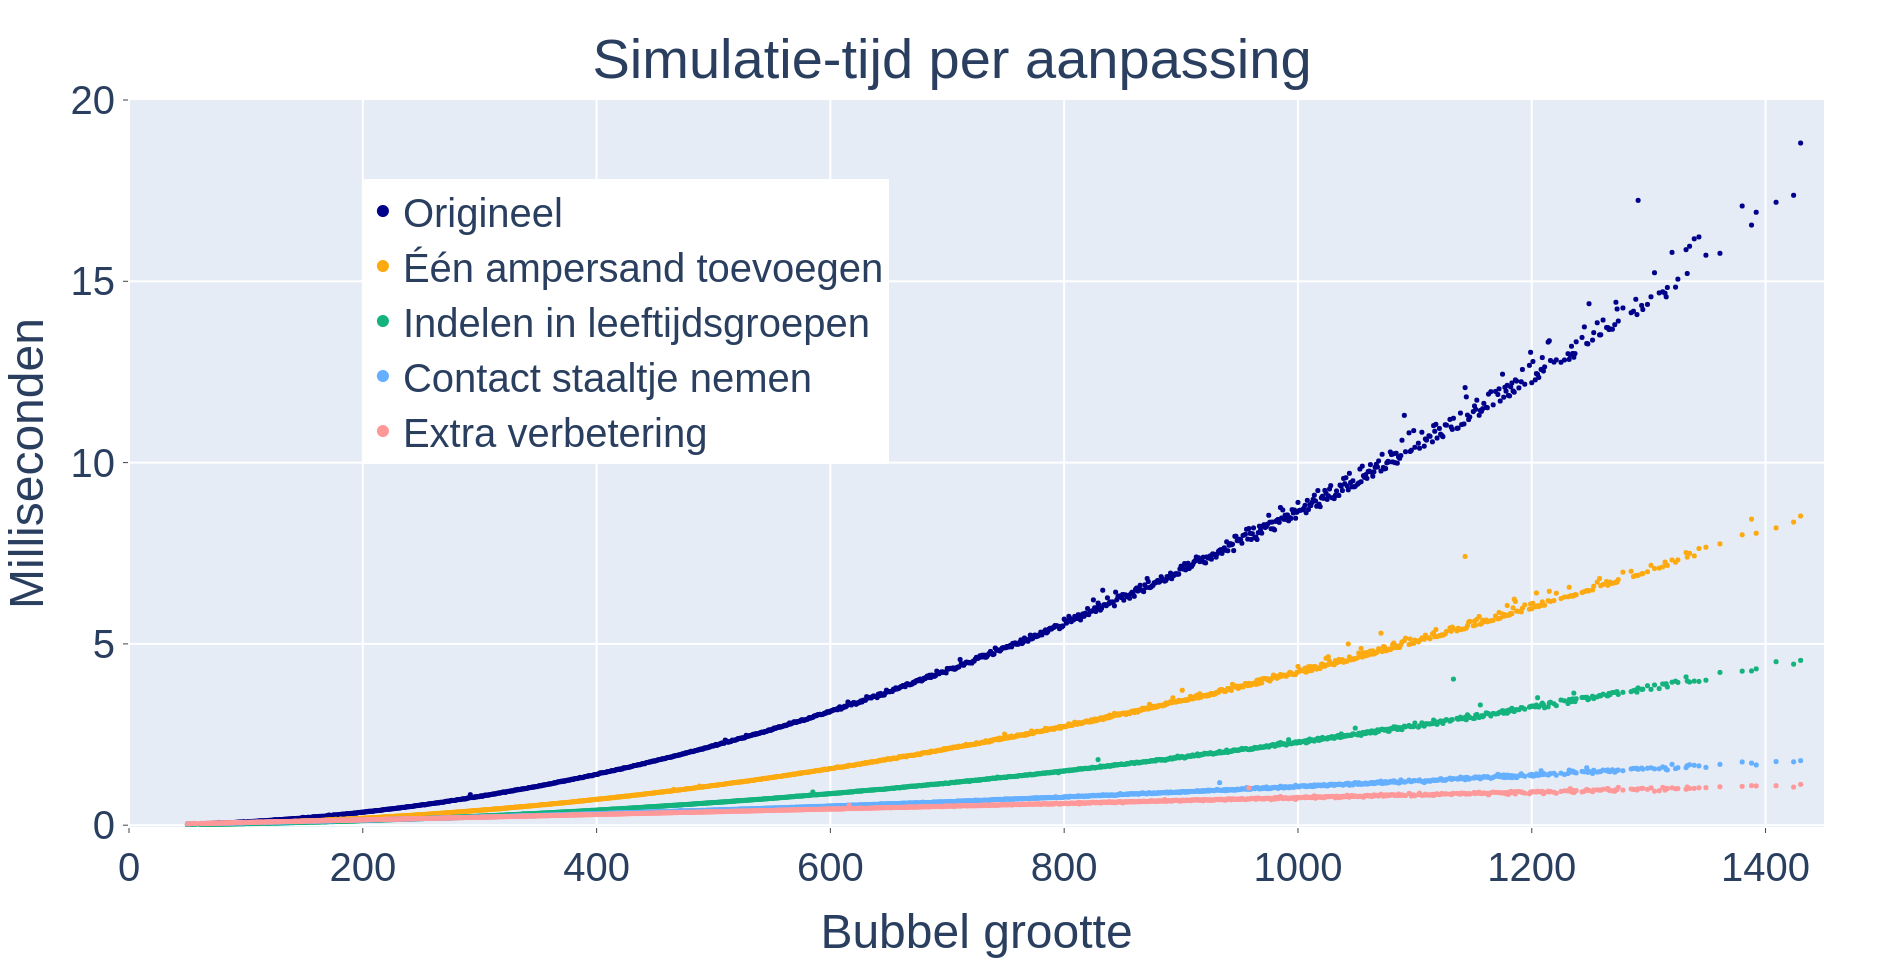
\includegraphics[width=\linewidth]{simulatietijd.png}

\subsection*{Een nieuwe taal ontwikkelen}
Naast het versnellen van de simulatie, heb ik nog een nieuwe computertaal ontwikkeld waardoor iedereen nu een simulatie kan uitvoeren. Het enige wat u hiervoor moet doen is in een paar regels beschrijven wat de simulatie voor u moet doen. Onderzoekers moeten hierdoor geen uitgebreide kennis hebben van het programma en kunnen meteen aan de slag. Een nieuwe taal creëren vergt echter zeer veel tijd om te implementeren en te onderzoeken. Mijn taal is daarom ook nog niet compleet, waardoor er komend academiejaar een thesis hierop verder gaat.

\end{document}
